\documentclass{beamer}
\usepackage{graphicx}
\usepackage{booktabs}
\usepackage{siunitx}
\usepackage{adjustbox}
\title{Concolic Testing of Mini from Scala}
\author{PACT:\\  Ricky Escobar \and Andrew Gilbert \and Andrew Tran}
\begin{document}
\begin{frame}
  \maketitle
\end{frame}
\begin{frame}{Overview}
  \begin{enumerate}
    \item Demo
    \item What we built
    \item Performance
  \end{enumerate}
\end{frame}

\begin{frame}{Demo}
\end{frame}

\begin{frame}{What we built}
  Uses algorithm from ``CUTE: A Concolic Unit Testing Engine for C''
  \begin{itemize}
    \item<2-> Every time the program is run, it gathers constraints from all
      branches taken
    \item<3-> It solves for inputs to go the other direction on each branch
    \item<4-> It adds the new inputs to the list of inputs to try
  \end{itemize}
\end{frame}

\begin{frame}
  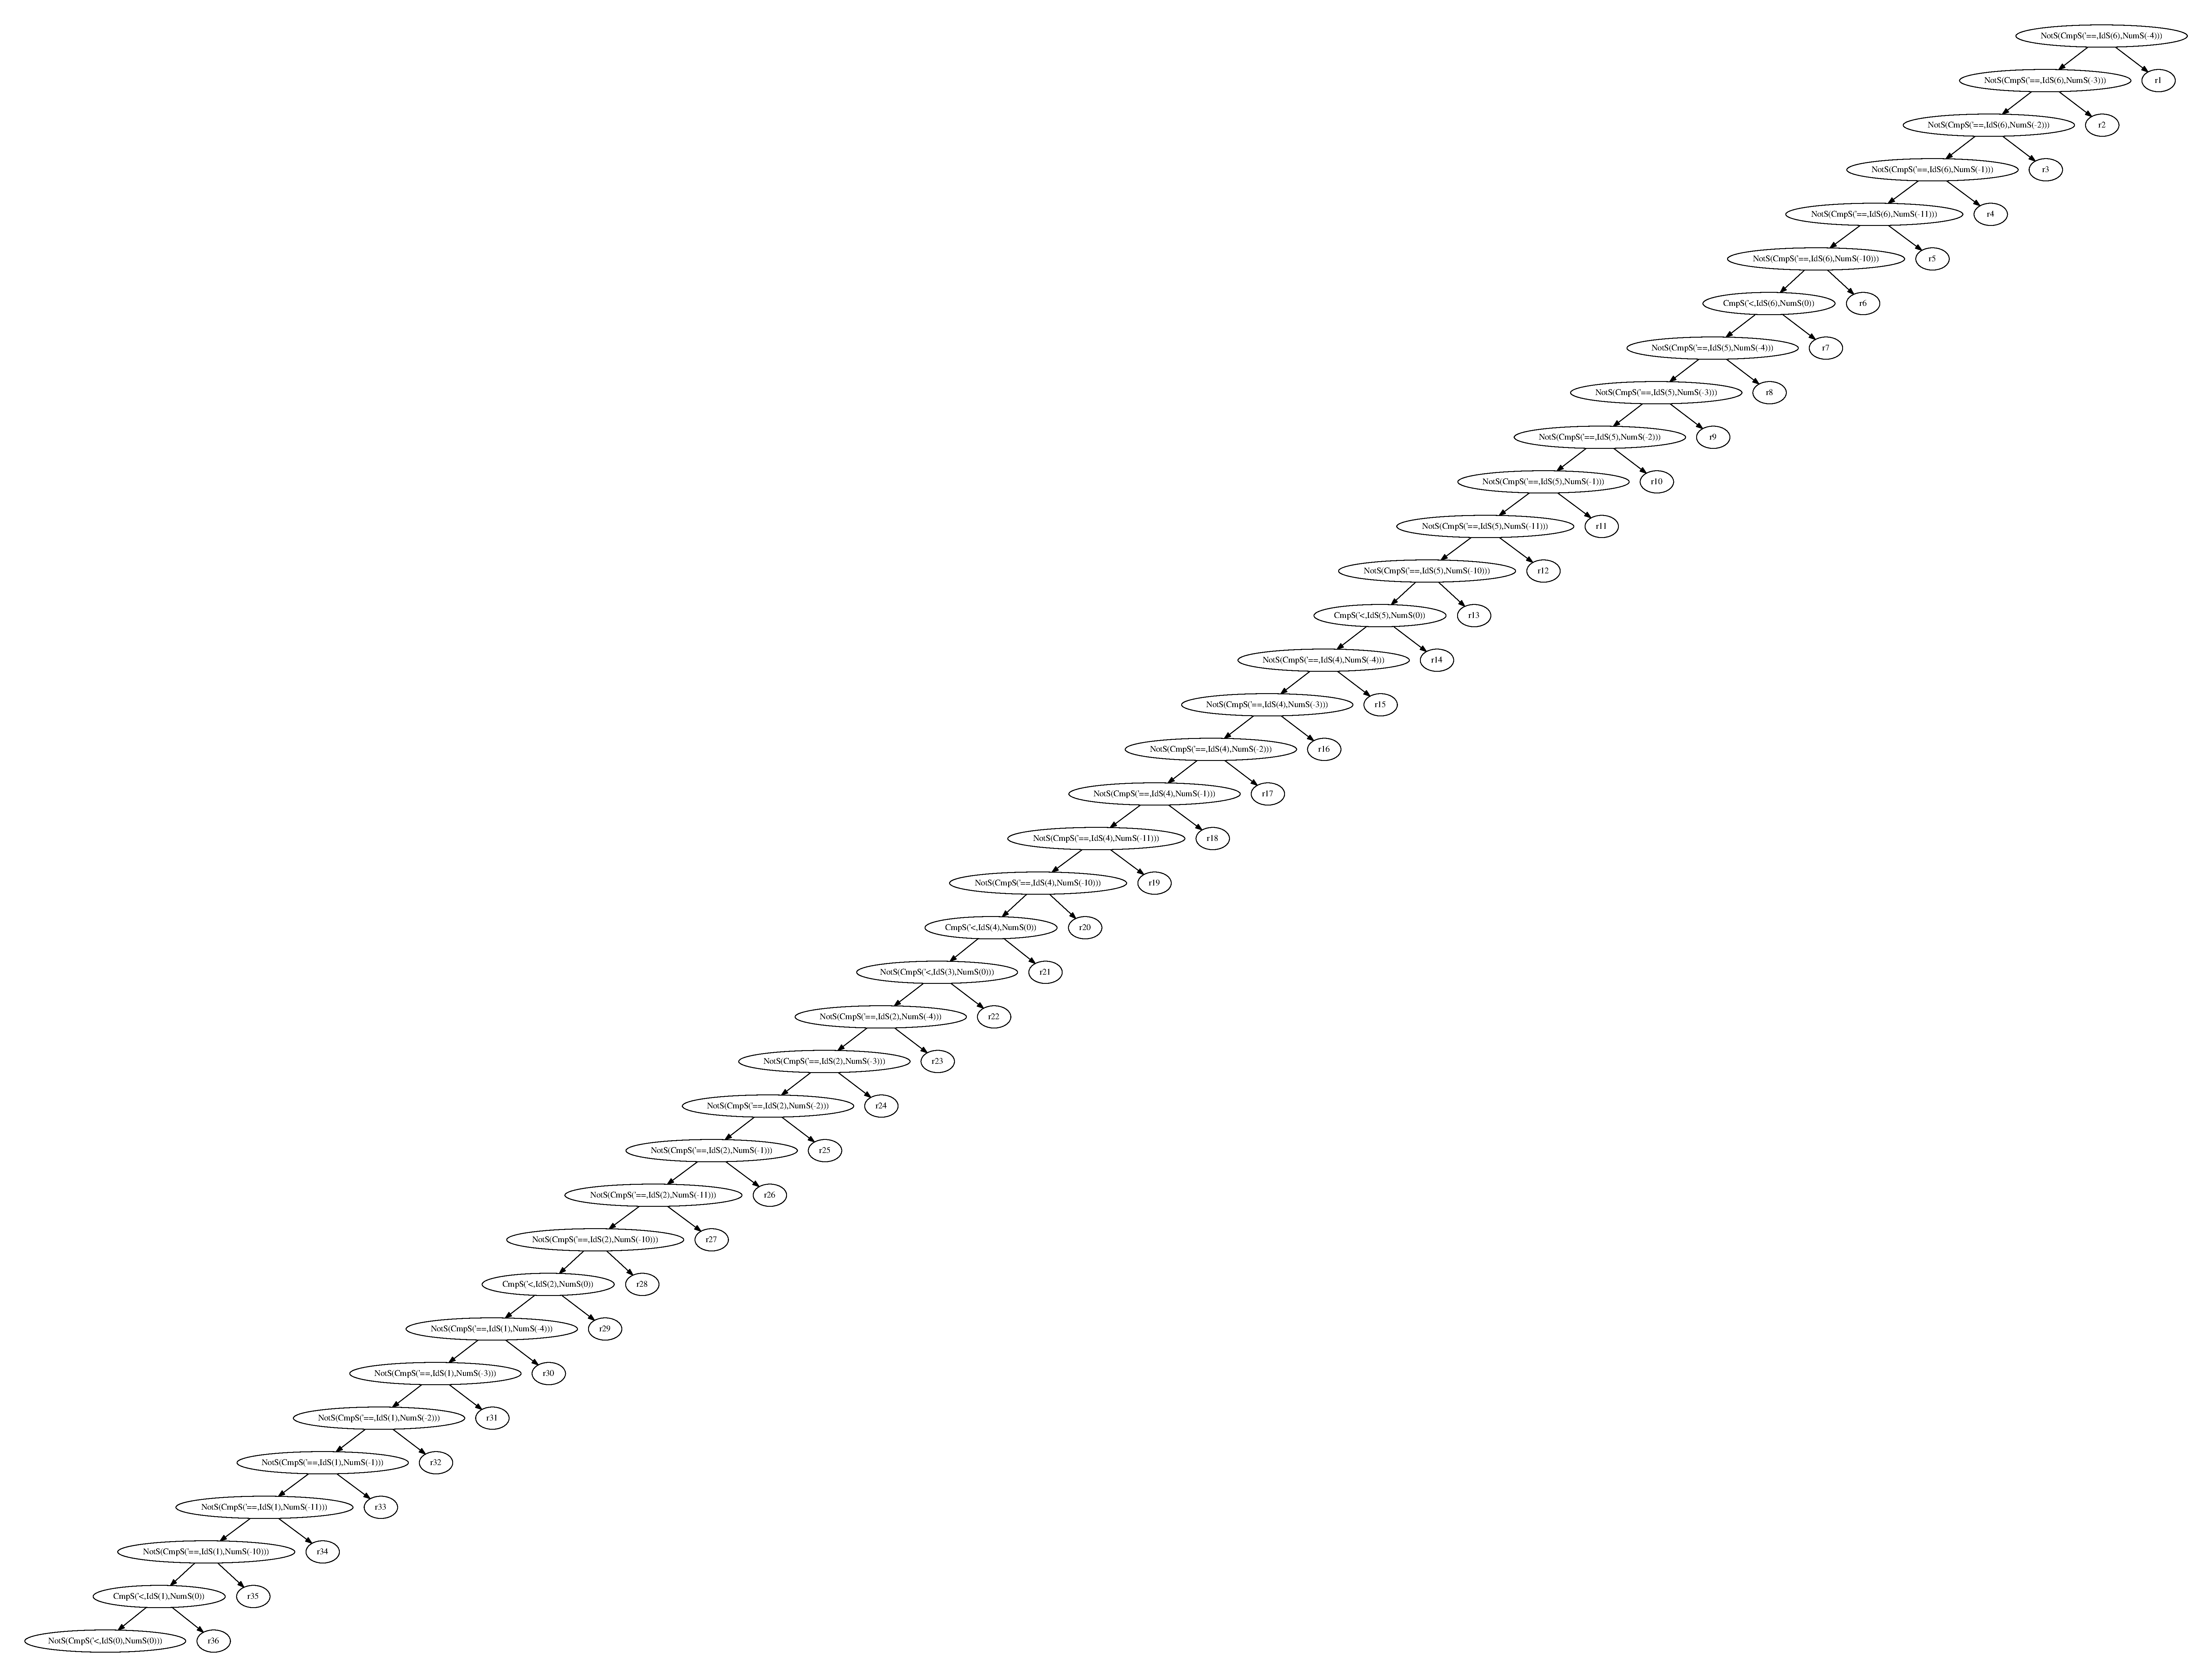
\includegraphics[height=\textheight,width=\textwidth,keepaspectratio]{iteration0}
\end{frame}

\begin{frame}
  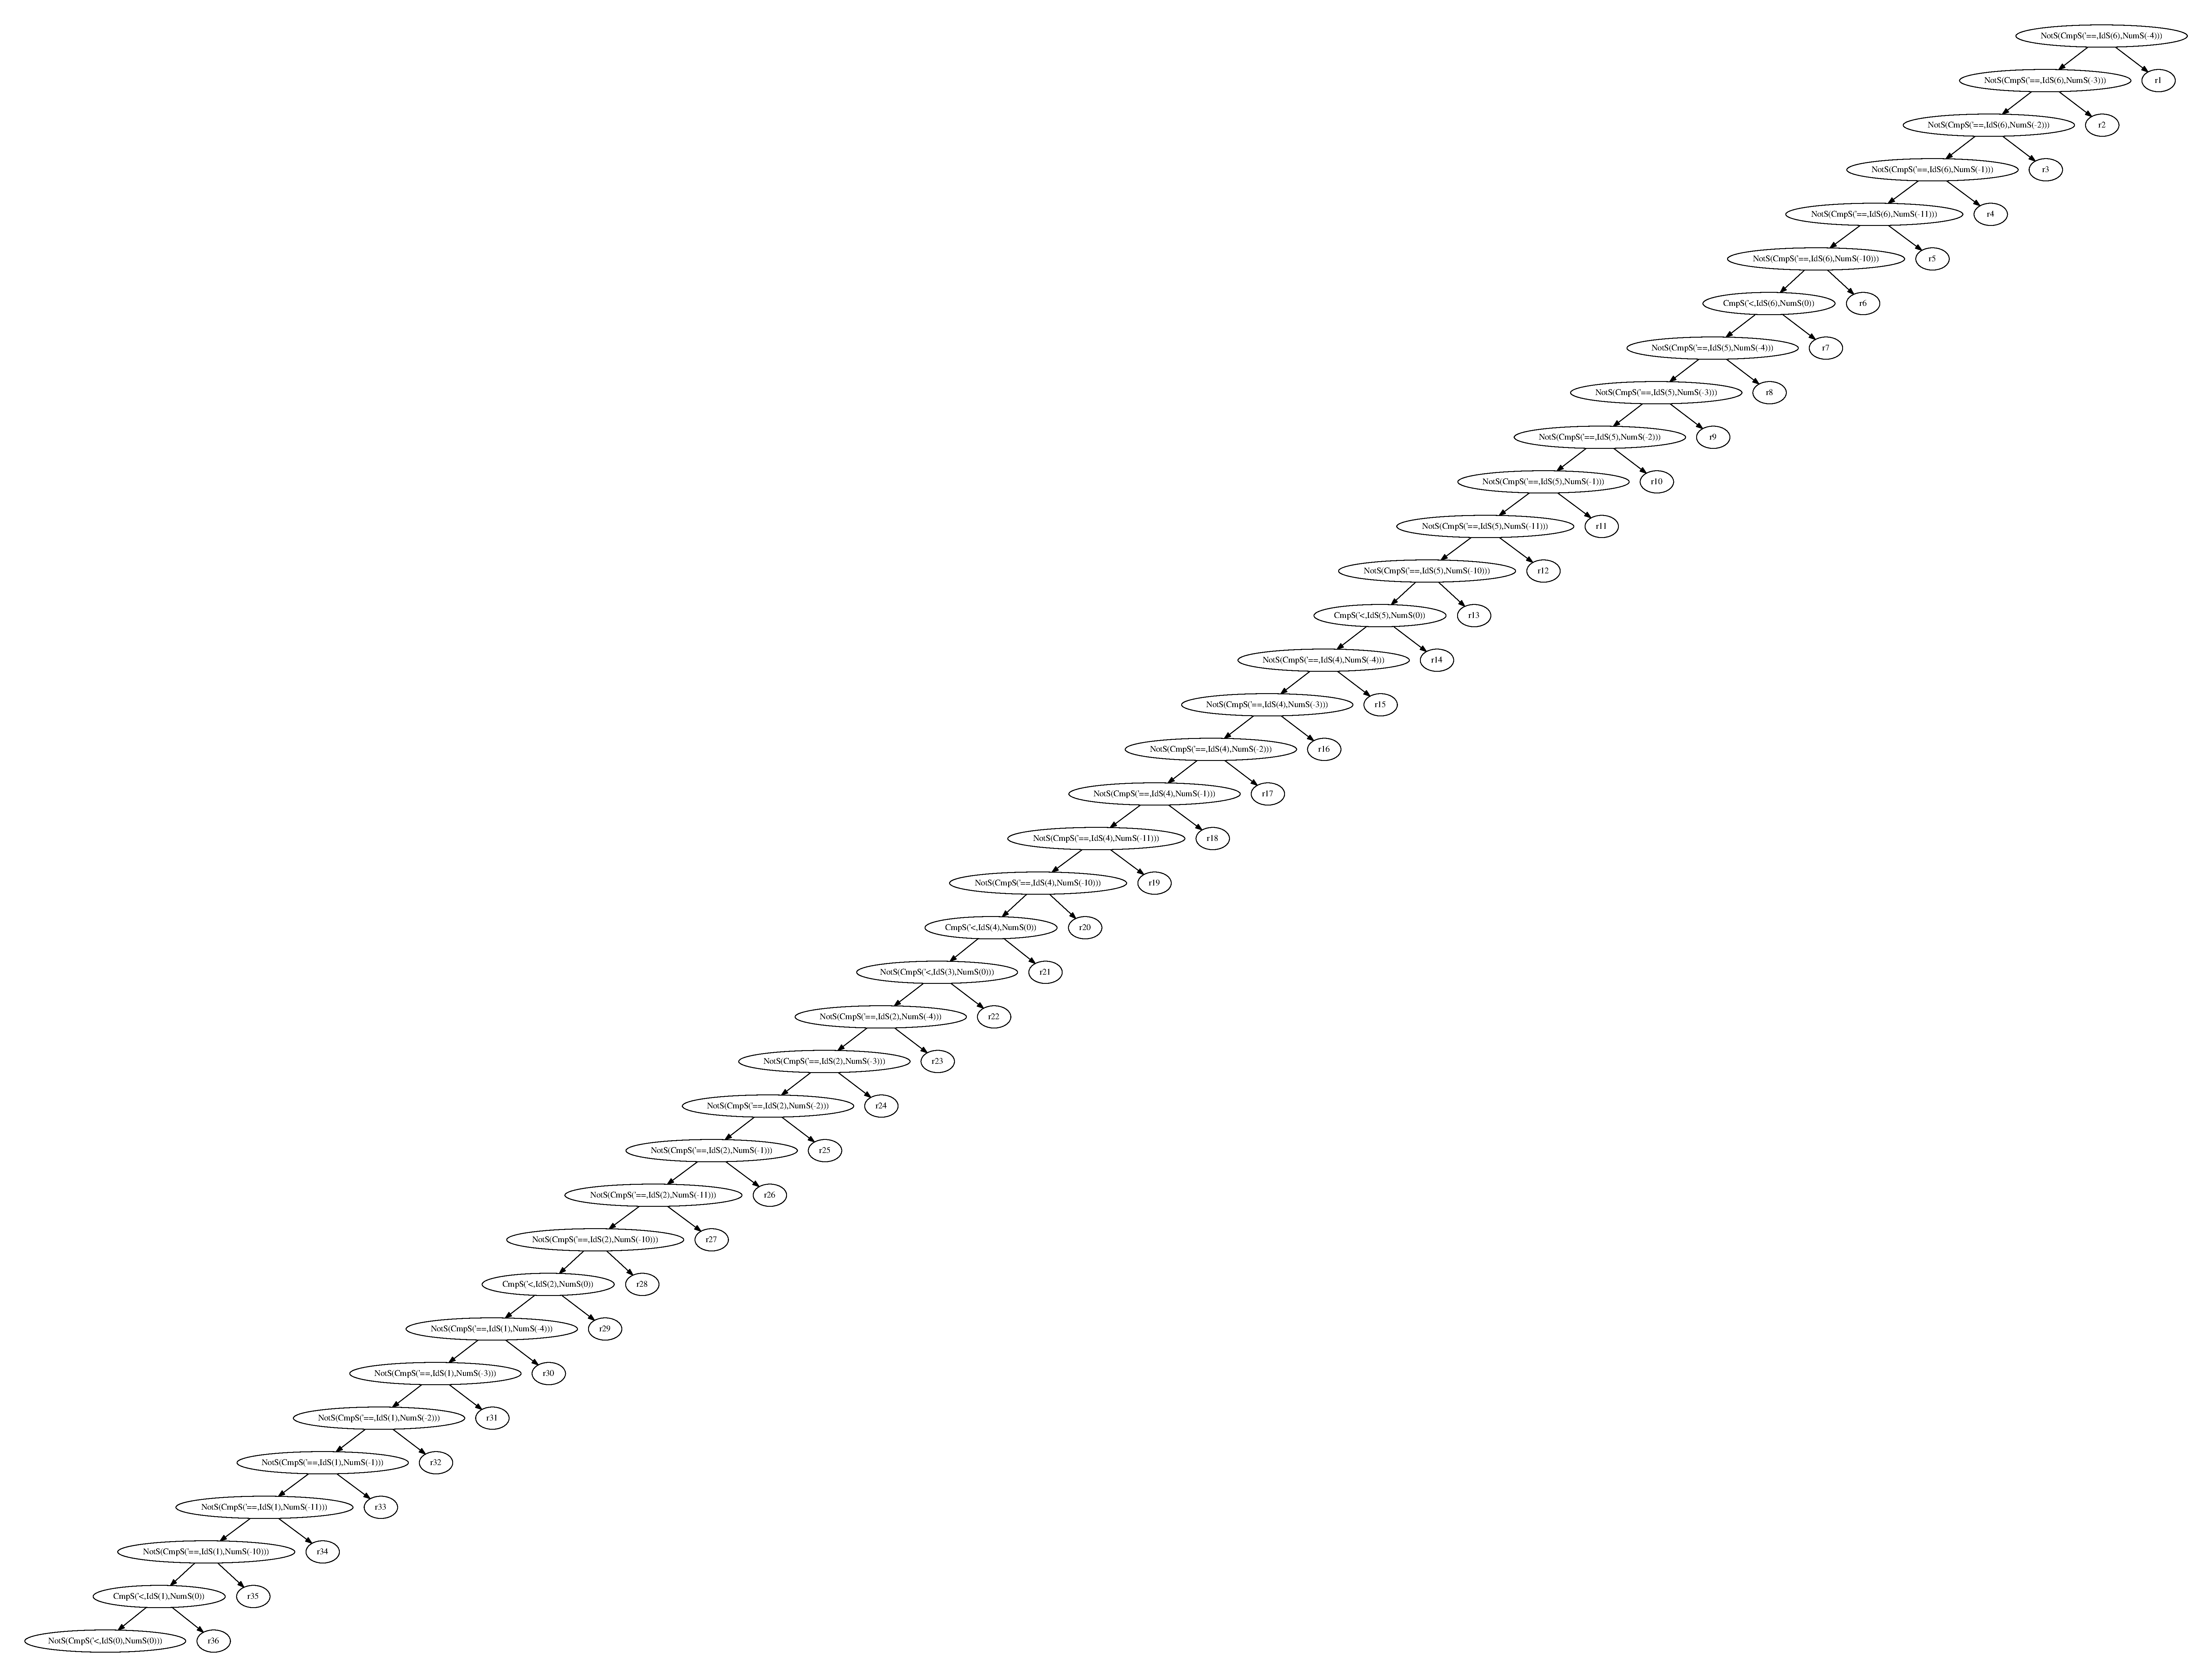
\includegraphics[height=\textheight,width=\textwidth,keepaspectratio,viewport=40in 30in 49in 37in]{iteration0}
\end{frame}

\begin{frame}{Performance (over three runs)}
  %\tiny
  %\begin{tabular}{ll|l|lll}
  %                            &            & Concolic Tester & \multicolumn{3}{c}{Fuzzer}\\
  %                            &            &                 & 50k Iterations               & Time-limited & Iteration limited\\
  %  \midrule
  %  \texttt{demo.mini}        & Time       & \SI{7.23}{s}    & \SI{10.00}{s}                & \SI{7.56}{s} & \SI{1.22}{s}\\
  %                            & Iterations & 1,344           & 50,000                       & 35,810       & 1,344\\
  %                            & Coverage   & 100\%           & 98.37\%                      & 95.12\%      & 74.80\%\\
  %  \midrule
  %  \texttt{draw.mini}        & Time       & \SI{0.64}{s}    & \SI{10.25}                   & \SI{0.98}{s} & \SI{0.42}{s}\\
  %                            & Iterations & 16              & 50,000                       & 733          & 16\\
  %                            & Coverage   & 100\%           & 100\%                        & 100\%        & 100\%
  %\end{tabular}
  \begin{adjustbox}{minipage=[c]{\pagewidth-.25in},center}
    \fontsize{10pt}{12pt}\selectfont
    \begin{tabular}{l|l|lll}
      & Concolic Tester & \multicolumn{3}{c}{Fuzzer}\\
                                                      &                 & 50k Iterations               & Time-limited & Iteration limited\\
      \midrule
      \multicolumn{5}{c}{\texttt{demo.mini}}        \\
      Time                                              & \SI{7.23}{s}    & \SI{10.00}{s}                & \SI{7.56}{s} & \SI{1.22}{s}\\
                               Iterations             & 1,344           & 50,000                       & 35,810       & 1,344\\
                               Coverage               & 100\%           & 98.37\%                      & 95.12\%      & 74.80\%\\
      \midrule
      \multicolumn{5}{c}{\texttt{draw.mini}}         \\
      Time                                              & \SI{0.64}{s}    & \SI{10.25}                   & \SI{0.98}{s} & \SI{0.42}{s}\\
                               Iterations             & 16              & 50,000                       & 733          & 16\\
                               Coverage               & 100\%           & 100\%                        & 100\%        & 100\%
    \end{tabular}
  \end{adjustbox}
  % \begin{tabular}{lll}
  %                             &            & Concolic Tester \\
  %   \midrule
  %   \texttt{demo.mini}        & Time       & \SI{7.23}{s}    \\
  %                             & Iterations & 1,344           \\
  %                             & Coverage   & 100\%           \\
  %   \midrule
  %   \texttt{draw.mini}        & Time       & \SI{0.64}{s}    \\
  %                             & Iterations & 16              \\
  %                             & Coverage   & 100\%          \\ 
  % \end{tabular}
  % \begin{tabular}{lllll}
  %                             &            & \multicolumn{3}{c}{Fuzzer}\\
  %                             &            & 50k Iter.               & Time-limited & Iteration limited\\
  %   \midrule
  %   \texttt{demo.mini}        & Time       & \SI{10.00}{s}                & \SI{7.56}{s} & \SI{1.22}{s}\\
  %                             & Iterations & 50,000                       & 35,810       & 1,344\\
  %                             & Coverage   & 98.37\%                      & 95.12\%      & 74.80\%\\
  %   \midrule
  %   \texttt{draw.mini}        & Time       & \SI{10.25}                   & \SI{0.98}{s} & \SI{0.42}{s}\\
  %                             & Iterations & 50,000                       & 733          & 16\\
  %                             & Coverage   & 100\%                        & 100\%        & 100\%
  % \end{tabular}
\end{frame}
% \begin{verbatim}
% [{:name=>{:tester=>"Fuzzer", :file=>"./draw.mini 16", :desc=>1},
% :time=>0.428060989,
% :coverage=>(1/1),
% :iters=>16},
% 
% {:name=>{:tester=>"Fuzzer", :file=>"./demo.mini 1344", :desc=>1},
% :time=>1.2299641226666669,
% :coverage=>(92/123),
% :iters=>1344},
% 
% {:name=>{:tester=>"Fuzzer", :file=>"./draw.mini 50000 0.64", :desc=>1},
% :time=>0.981448018,
% :coverage=>(1/1),
% :iters=>733},
% 
% {:name=>{:tester=>"Fuzzer", :file=>"./demo.mini 50000 7.23", :desc=>1},
% :time=>7.561110392000001,
% :coverage=>(39/41),
% :iters=>35810}]
% 
% [{:name=>{:tester=>"ConcolicTester", :file=>"./draw.mini", :desc=>1},
% :time=>0.6356207603333334,
% :coverage=>(1/1),
% :iters=>16},
% 
% {:name=>{:tester=>"ConcolicTester", :file=>"./demo.mini", :desc=>1},
% :time=>7.229123219000001,
% :coverage=>(1/1),
% :iters=>1344},
% 
% {:name=>{:tester=>"Fuzzer", :file=>"./draw.mini 50000", :desc=>1},
% :time=>10.248840253,
% :coverage=>(1/1),
% :iters=>50000},
% 
% {:name=>{:tester=>"Fuzzer", :file=>"./demo.mini 50000", :desc=>1},
% :time=>10.001355685666669,
% :coverage=>(121/123),
% :iters=>50000}]
% 
% \end{verbatim}

\end{document}
